\newpage
\section{Introduction}
\qquad Battleship (also known as Battleships or Sea Battle) is a strategy type guessing game for two players. It is played on ruled grids (paper or board) on which each player's fleet of warships are marked. The locations of the fleets are concealed from the other player. Players alternate turns calling "shots" at the other player's ships, and the objective of the game is to destroy the opposing player's fleet. \\[6pt]

\begin{figure}[H]
    \centering
    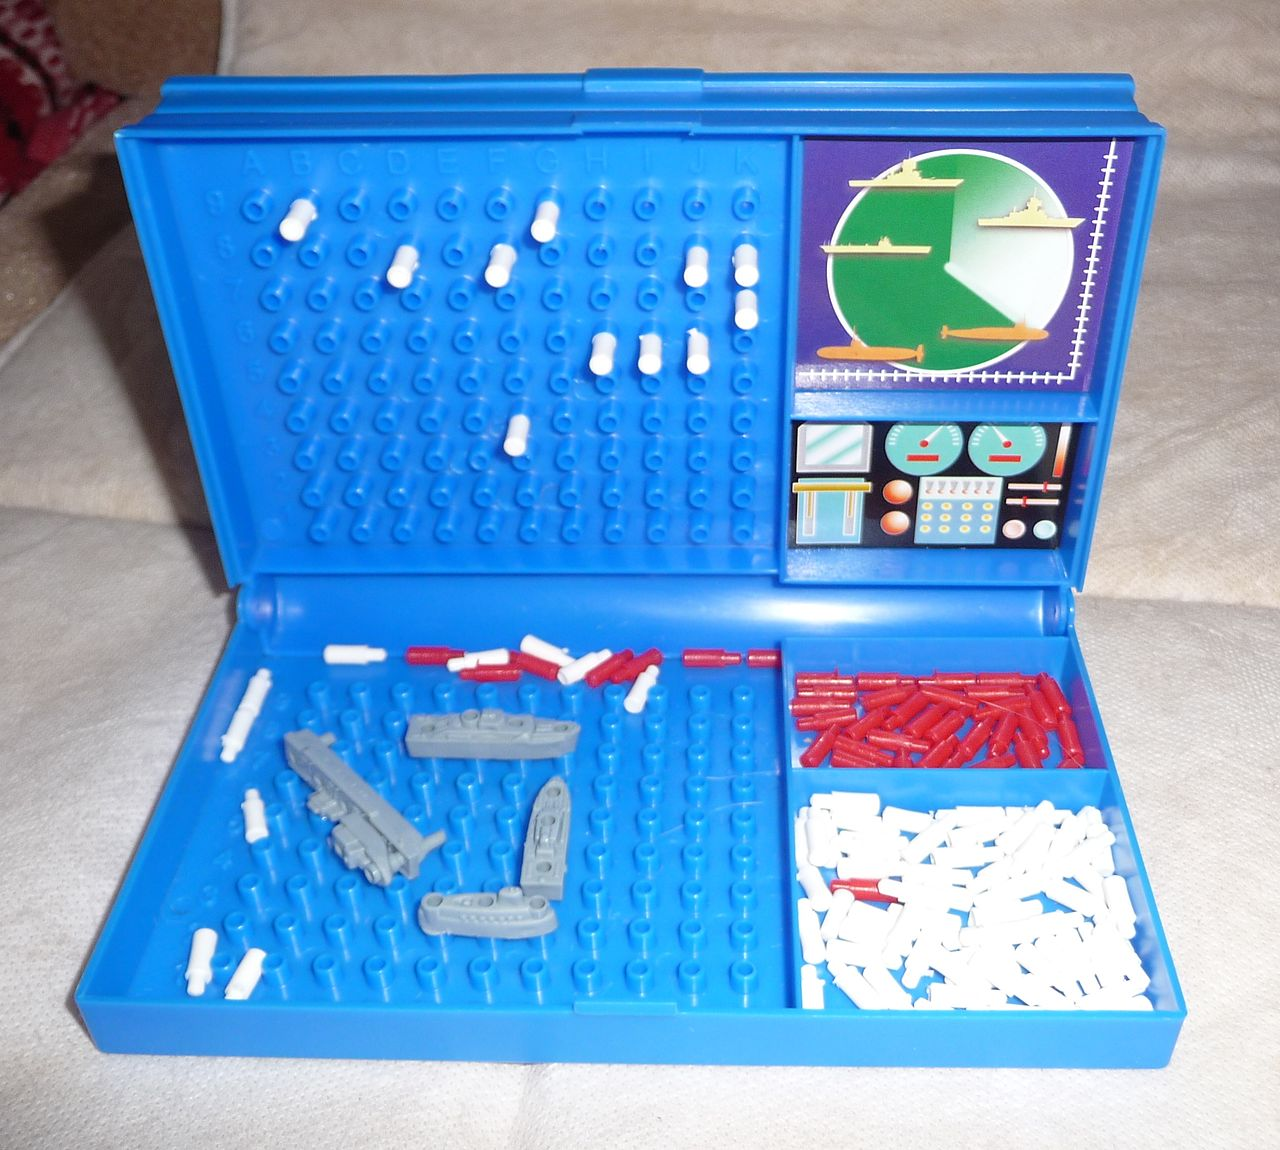
\includegraphics[width=12cm]{graphics/battleship.jpg}
    \selectlanguage{english}
    \caption{Example of the classic battleship game}
\end{figure}

\subsection{Description}
\qquad The game is played on four grids, two for each player. The grids are typically square - usually 10$\times$10 - and the individual squares in the grid are identified by letter and number. On one grid the player arranges ships and records the shots by the opponent. On the other grid, the player records their own shots.\\

\qquad Before play begins, each player secretly arranges their ships on their primary grid. Each ship occupies a number of consecutive squares on the grid, arranged either horizontally or vertically. The number of squares for each ship is determined by the type of ship. The ships cannot overlap (i.e., only one ship can occupy any given square in the grid). The types and numbers of ships allowed are the same for each player. These may vary depending on the rules. The ships should be hidden from players sight and it's not allowed to see each other's pieces. The game is a discovery game which players need to discover their opponents ship positions.\\

\qquad After the ships have been positioned, the game proceeds in a series of rounds. In each round, each player takes a turn to announce a target square in the opponent's grid which is to be shot at. The opponent announces whether or not the square is occupied by a ship. If it is a "hit", the player who is hit marks this on their own or "ocean" grid (with a red peg in the pegboard version), and announces what ship was hit. The attacking player marks the hit or miss on their own "tracking" or "target" grid with a pencil marking in the paper version of the game, or the appropriate color peg in the pegboard version (red for "hit", white for "miss"), in order to build up a picture of the opponent's fleet.\\

\qquad If all of a player's ships have been sunk, the game is over and their opponent wins.